\chapter{Designing the System}
	In the following chapter, the overall design of the system is discussed. First and foremost, the basic architechture is decided, based on the requirements. Then more detailed subjects are covered, such as how authentication will work, how the solution keeps the users' data safe, and generally how it will work under the hood - so to speak.

	\section{Architecture}
		\label{sec:arch}
		As per the requirements specified in section \ref{sec:requirements} on page \pageref{sec:requirements} the solution will have to be distributed. As such, there are two primary basic paradigms which can be used: Peer-to-Peer and Client-Server. In the following sections the pros and cons of the two will be discussed, and a conclusion of which is more beneficial for the project will be made.

		\begin{figure}
			\centering
			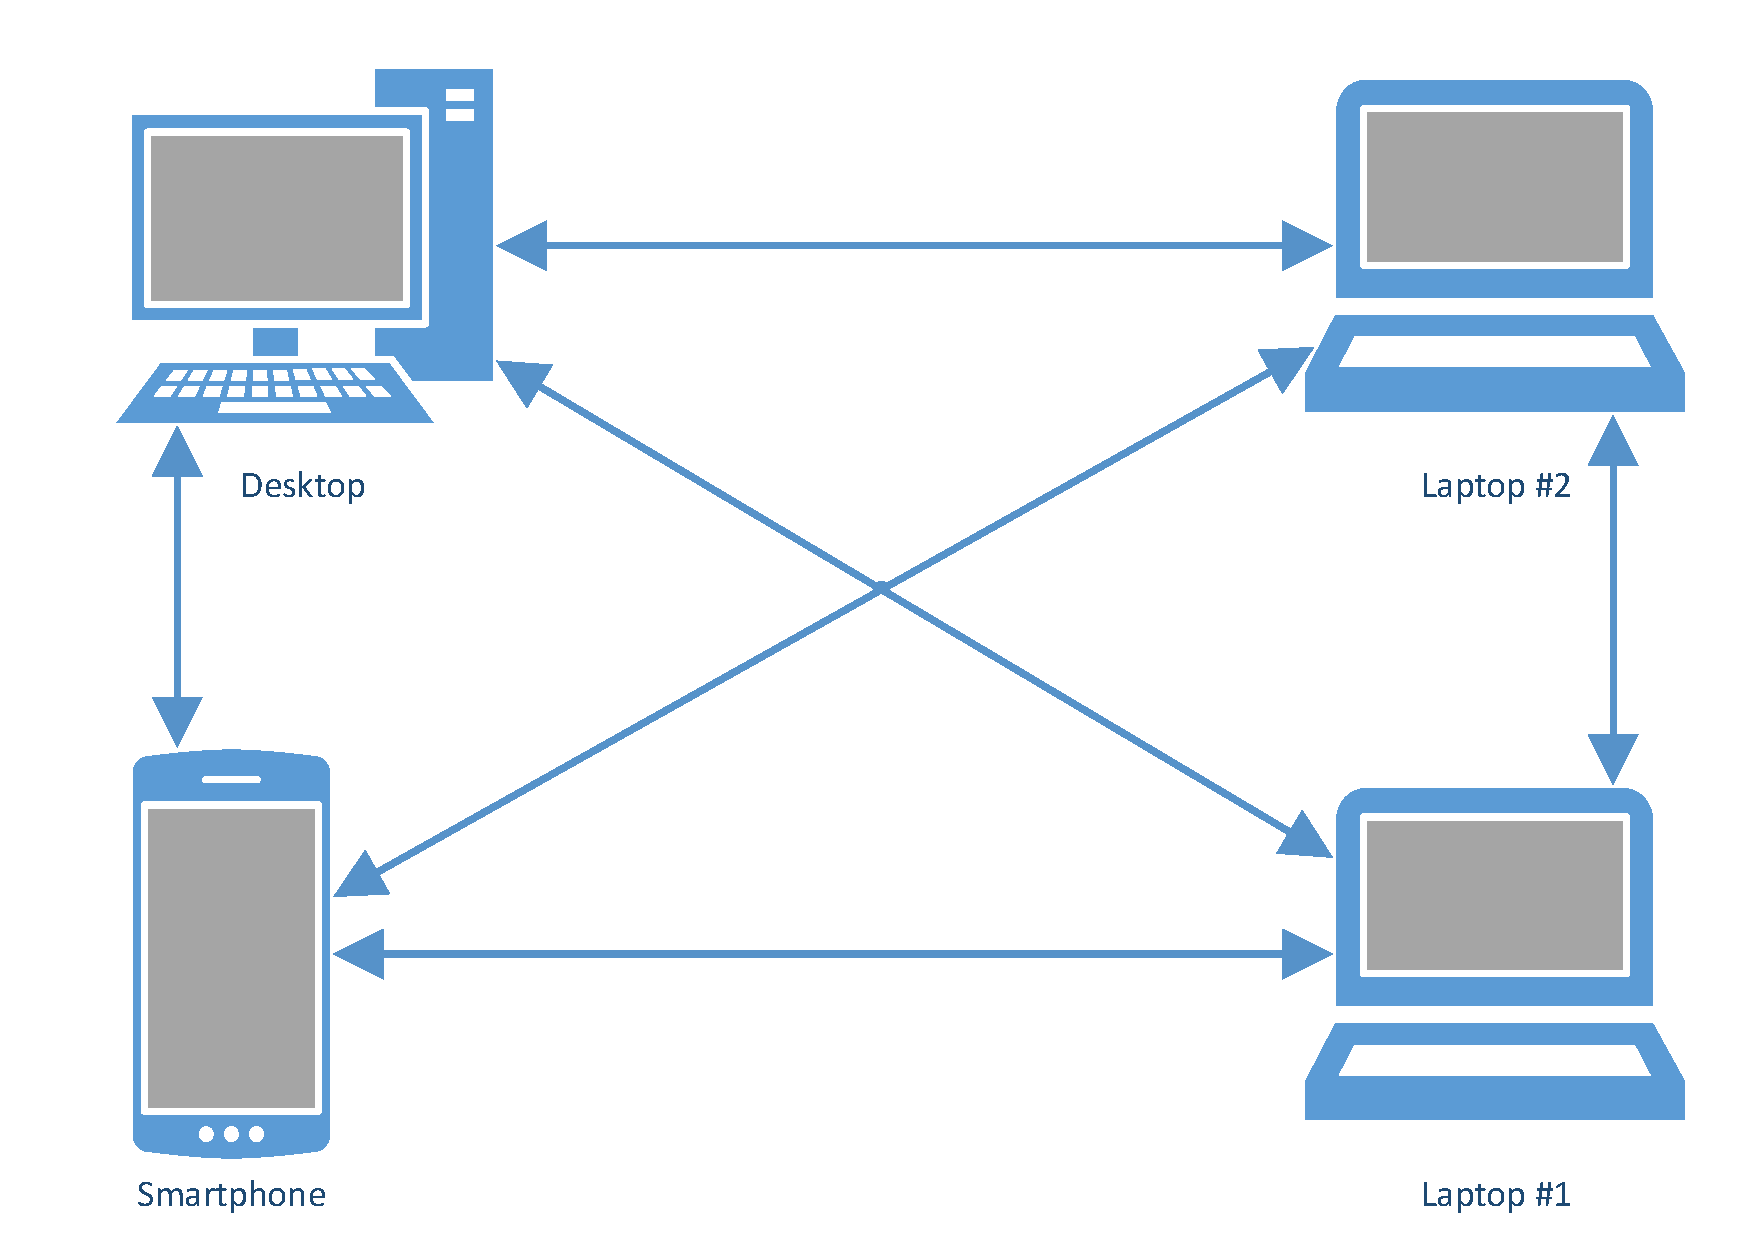
\includegraphics[width=\textwidth]{figures/design/PeerToPeer.pdf}
			\caption{Peer-to-Peer structure visualised.}
			\label{fig:peertopeer}
		\end{figure}

		\begin{figure}
			\centering
			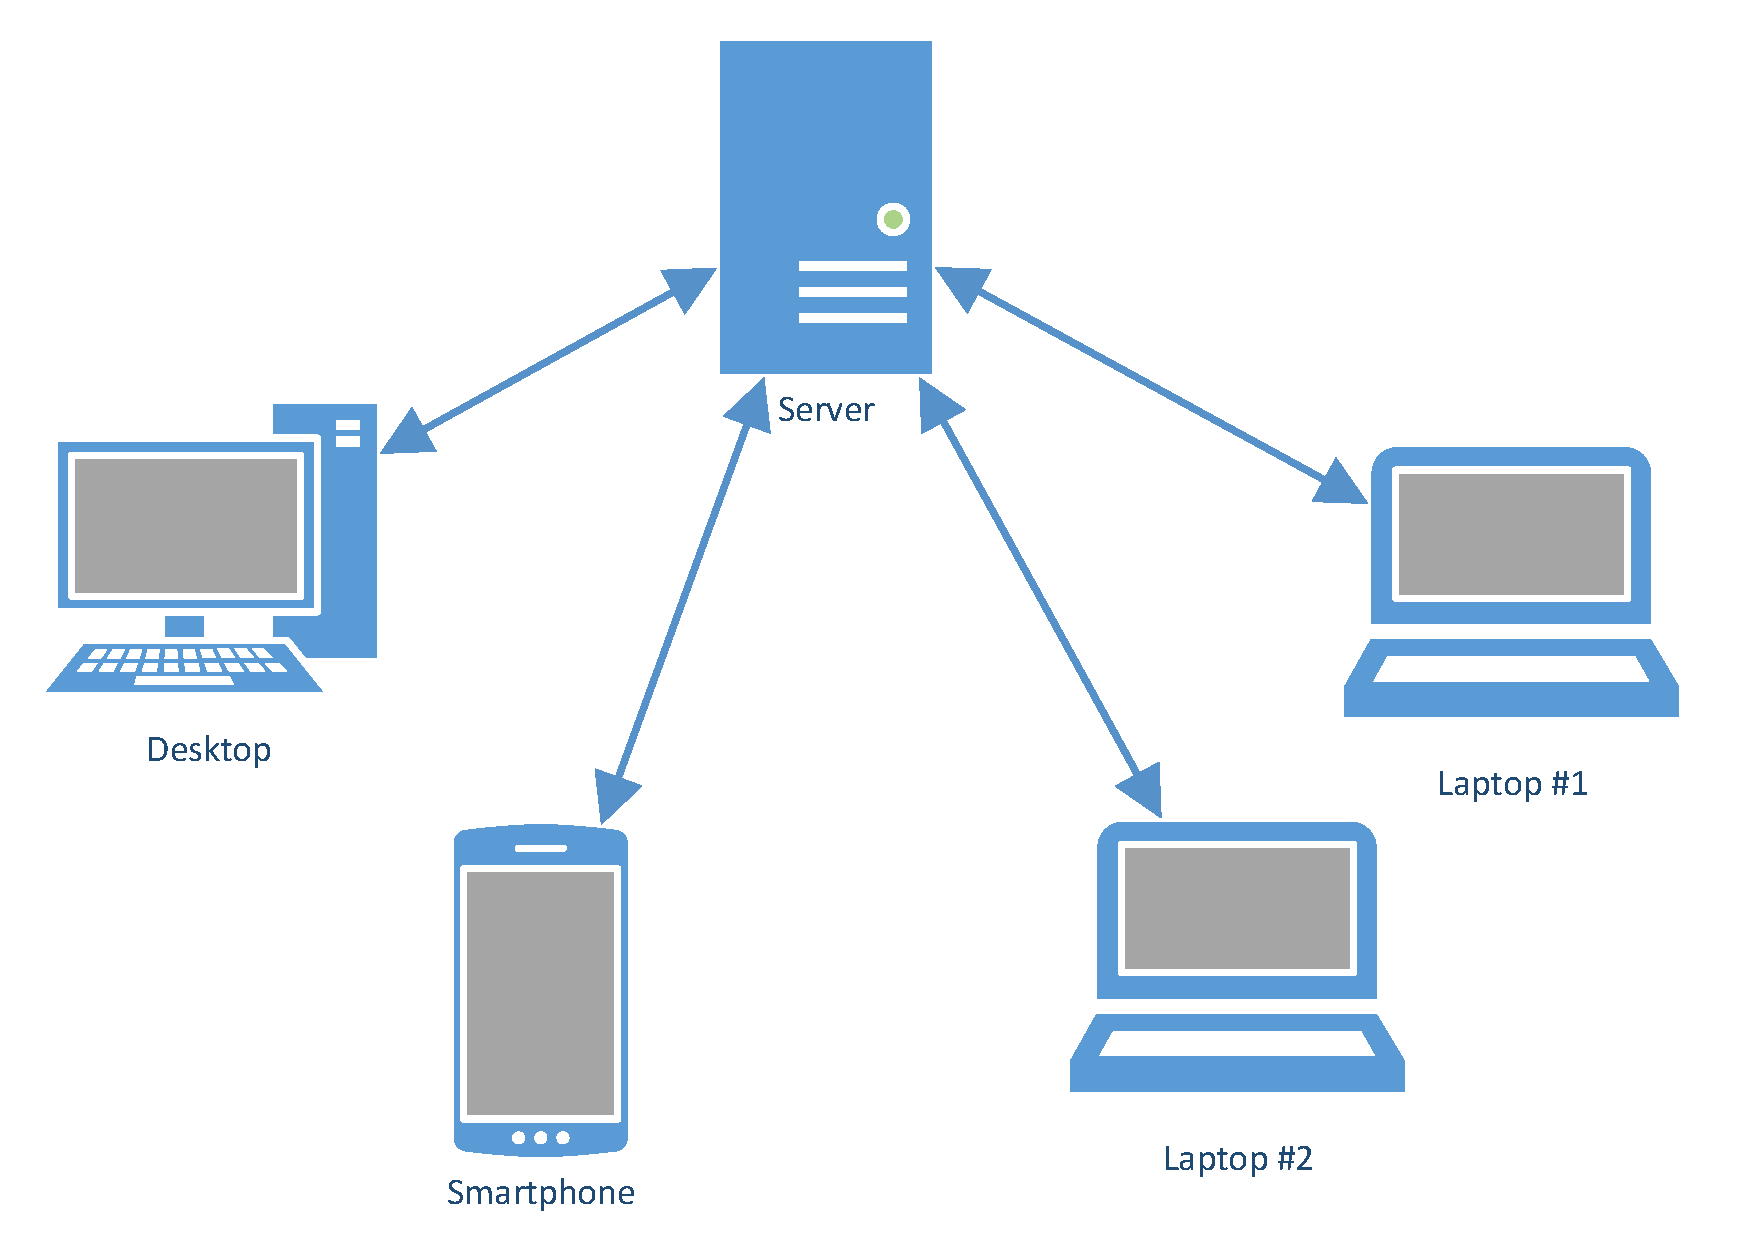
\includegraphics[width=\textwidth]{figures/design/ClientServer.pdf}
			\caption{Client-Server structure visualised.}
			\label{fig:clientserver}
		\end{figure}


		\subsection{Peer-to-Peer}
			Over the past few years, peer-to-peer technology has become ever so more appealing to the masses. Applications such as BittorrentSync applies peer-to-peer technology in an effort to synchronise data between devices. Such an approach could easily be adapted to the problem at hand. A number of a user's devices are online, and synchronises a local password database file between themselves, as visualised on figure \ref{fig:peertopeer} on page \pageref{fig:peertopeer}. This file is then accessed through a native application, on the target device. 

			This approach \emph{definitely} has the lowest overhead of the two: After all it is only devices that needs to have access to the passwords, that need to be setup, maintained, and running for it to be used. However, it does have some drawbacks. Most noticeable, that a native application is required for it to work. This means that for \emph{all} platforms an application needs to be developed. This, in returns, results in a much larger codebase, higher risk of bugs, and a risk of lower consistency across devices. Furthermore, the requirements of logging, as per section \ref{sec:requirements} on page \pageref{sec:requirements}, becomes a lot more difficult, if not to say impossible.

			Additionally, there is a pitfall using this approach. The synchronization requires at least \emph{one} peer with the newest version, to be online for it to work. Let us imagine a user, Paul. Paul has three devices he wish to synchronize passwords to: A desktop, a laptop, and a smartphone -- a very common scenario! Before leaving for a holiday, Paul updates a password on his desktop, while his laptop is closed. Since the smartphone is online at the time, the password is stored there and Paul is perfectly able to access it on his way to the airport. Since it's a long trip, Paul's smartphone runs out of battery along the way. ``No problem!'', Paul thinks and pulls out his laptop -- but oh no! Since the laptop has been offline ever since he left home, it has not received the updated password. And since it is the only online peer -- the desktop at home is turned off and the smartphone has run out of battery -- he can't fetch the newest version. 

			The scenario presented before, can be somewhat mitigated by creating an ``always on peer''. It is a peer in the network, which is always connected and thus always has the newest version available for other peers. However, doing this very much negates one of the strongest arguments \emph{for} this approach: The lower overhead.

		\subsection{Client-Server}
			The client-server paradigm has been the basic model used, since the dawn of the modern internet. When browsing facebook, accessing gmail, or posting a tweet, this is the paradigm employed. It is also the most widespread model used, by the solutions examined in chapter \ref{chap:analysis}.

			Using this approach, there would have to be a dedicated server, acting as the ``master storage'' of passwords. Each client then connects to this server and fetches the passwords. This type of connection is visualised on figure \ref{fig:clientserver} on page \pageref{fig:clientserver}. This does, however, come with its own drawbacks. Since all passwords are stored on a single server, it introduces the risk of a single point of failure. Should the server be compromised or is otherwise unavailable, passwords can not be retrieved \emph{(unless a local cache is used, but this is delving into implementation details)}. It also comes with overhead in form of cost and maintenance. A server will have to be maintained and run 24/7. However, as mentioned in section \ref{sec:privatecloud_cost} on page \pageref{sec:privatecloud_cost}, this can be achieved using low-power devices such as a Raspberry Pi, reducing the financial cost significantly.

			Finally, using the client-server paradigm counters the scenario presented in the previous section. When Paul updates the password from home, the updated password is stored on the server. When he uses his laptop, after his phone has died, it will fetch the updated password from the server.


		\subsection{Conclusion}
			After having weighed the pros and cons of the two approaches, it is decided that a classic client-server architecture will be used. It is deemed that it will create a more seamless experience for the user, and over all will be a more robust solution.

			Another argument why the client-server paradigm is preferable is that if the peer-to-peer paradigm is used, a native application is \emph{required}. This is not the case for the client-server paradigm. A web UI could serve as a front-end, creating a completely identical user experience across devices. But a native application could also be the solution, for the client-server application. Hence, this paradigm allows more freedom of implementation, than peer-to-peer does.

			From here on out, the solution will be split into two parts: The front-end \emph{(client)} and back-end \emph{(server)} -- two very common denominators.

	\section{Communicating}
		\label{sec:comms}
		Having determined that the solution will be using the client-server paradigm, the next task is to determine how front-end and the back-end will communicate. There are a number of different available technologies and protocols readily available for use in such a scenario.

		One important fact, that needs to be stated that the back-end is practically equivalent to a web service. As such, 

		\begin{itemize}
			\item Representational State Transfer
			\item SOAP	
			\item Sockets
			\item Remote Procedure Calls
		\end{itemize}

		\subsection{Remote Procedure Call}
			Remote Procedure Calls, or RPC for short, was introduced by Birrell and Nelson \cite{birell1984} in 1984. The basic concept is to hide the implementation details of invoking a method remotely, for the user.

			The core concept of RPC is that invoking remote methods, are no different than invoking a local method. When the program invokes this method, the underlying software then makes the remote call, hiding these details from the programmer. This is the supposed strength of RPC: It is exactly like invoking a local method.

			An example of an RPC method, could be a method to get a user's data:
			\begin{verbatim}
				getUser(<ID>)
			\end{verbatim}

			For simplicity purposes, Remote Method Invocation is considered equivalent to RPC. Likewise implementations of RPC such as XML-RPC, Corba, and so forth, are considered under the same umbrella.

		\subsection{Representational State Transfer}
			Representational State Transfer, or REST for short, was introduced by Fielding and Taylor \cite{Fielding:2000:PDM:337180.337228} in 2000. REST is an architecture style for designing networked application. It is a stateless, client-server communication \emph{style}, which in most cases uses the Hypertext Transfer Protocol \emph{(HTTP)} protocol and the accompanying HTTP ``verbs''. Traditionally REST uses JSON as body encoding, however it is also possible to use XML.

			The core notion of REST is that resources are bundled in collections, on which the HTTP verbs are used. The API then exposes these collections as Uniform Resource Identifiers \emph{(URIs)} in what is commonly known as endpoints. Using the various HTTP verbs on these endpoints results in actions being invoked on said collections.

			These verbs are for example -- but not limited to-- \verb=GET=, \verb=POST=, \verb=PUT=, \verb=PATCH=, and \verb=DELETE=. These five verbs roughly translates to the basic CRUD operations, as listed on table \ref{tbl:verbs} on page \pageref{tbl:verbs}. So, for instance if one where to \verb=GET= the endpoint of \verb=/api/users= one would get the list of all users on the system. However, most of the time the distinction between \verb=PUT= and \verb=PATCH= is ignored, and \verb=PUT= is allowed to perform partial updates. Table \ref{tbl:rest_example} on page \pageref{tbl:rest_example} shows an example of an API on the \verb=users= resource, showing the result of the respective verbs and their payload. In the example the host of the endpoints have been removed, the prefix could for example be \verb=https://someapi.com/api=, so that an endpoint would be \verb=https://someapi.com/api/users=.

			\begin{table}
				\begin{tabular}{r|l}
					\verb=GET= 		& Read 				\\
					\verb=POST= 	& Create 			\\
					\verb=PUT= 		& Complete update 	\\
					\verb=PATCH= 	& Partial update 	\\
					\verb=DELETE= 	& Delete 			\\
				\end{tabular}

				\caption{How HTTP verbs maps to CRUD operations.}
				\label{tbl:verbs}

			\end{table}

			\begin{table}
				\begin{tabular}{p{0.15\textwidth} | p{0.30\textwidth} | p{0.15\textwidth} | p{0.25\textwidth}}
					Method & Request Body & Endpoint & Ouput \\
					\hline
					\verb=GET= & Empty & /api/users & List of all users \\
					\hline
					\verb=GET= & Empty & /api/users/1 & Details of user with ID of 1 \\
					\hline
					\verb=POST= & \{username:"Daniel", phone:"+45 88888888"\} & /api/users & Creates a new User with the name Daniel and the phone number +45 88888888 \\
					\hline
					\verb=PUT= & \{username:"John"\} & /api/users/1 & Updates the username of the user with ID of 1\\
					\hline
					\verb=DELETE= & Empty & /api/users/1 & Deletes the user with ID of 1\\
				\end{tabular}

				\caption{Example of HTTP verbs used on a REST API for the collection of users.}
				\label{tbl:rest_example}

			\end{table}

		\subsection{Simple Object Access Protocol}
			Simple Object Access Protocol \emph{(SOAP)} was developed by Goshein, Atkinson, Winer, and Box for Microsoft in 1997 \cite{soap_origin}. SOAP is considered an extension of XML-RPC and -- like its predecessor -- uses XML encoding. As implied by its successor SOAP is \emph{strictly speaking} considered an RPC, however due to its uniqueness from ``traditional'' RPCs it is considered separately.

			SOAP can be used with any number of protocols, due to its neutrality, however it is usually used with HTTP or SMPT. Web services relying on SOAP, usually publish a public definition of the available methods, using the Web Service Definition Language \emph{(WSDL)}. This can then be consumed by other clients, making integration with third parties much easier.

			Since SOAP used XML encoding, it is \emph{quite} verbose, and the pure data overhead is significant. Using the same example as from REST, getting the information for a user with ID 1 requires a rather large request body. the XML uses multiple namespaces, the \verb=xmlns= tags are required to define each of them, as \verb=SOAP= and \verb=m= respectively.

			\begin{verbatim}
				<SOAP:Envelope xmlns:SOAP="http://schemas.xmlsoap.org/soap/envelope/">
				    <SOAP:Body>
				        <m:getUser xmlns:m="https://someapi.com/api">
				            <userId>41</userId>
				        </m:getUser>
				    </SOAP:Body>
				</SOAP:Envelope>
			\end{verbatim}


		\subsection{Sockets}
			Underlying all of the previously described technologies are sockets. Sockets are the basic method computers communicate with eachother. Hence, of course it can be used for this purpose. However, there is a \emph{reason} the previous technologies exist: They take care of some of the heavy lifting. Defining a standard for communication, redundancy, standard errors, etc. are but some of the advantages of using either of the previously described technologies. As such, using sockets directly is dismissed without further arguments. 


		\subsection{Making A Choice}
			Making the final choice of how the solution will communicate is important. It sets limitation on future work, and could possibly influence design choices not yet even thought of. 

			First and foremost let us examine RPC. While it \emph{was} the go-to method for achieving the sort of communication which is needed in this project, the issue of implementation remains. Each platform will need its own unique implementation of whichever RPC standard that is chosen. And there is no guarantee that all of these will adhere to the specifications. Additionally, since its usage has become less widespread, it will also hinder further development and integration from third parties, down the line. As such, RPC is dismissed as a possible solution.

			This leaves SOAP and REST. SOAP is a very ``heavy'' tool, often used in commercial applications, due to its stricter nature. Because of the XML syntax, their payload is \emph{significantly} larger than that of REST using JSON. This results in SOAP being magnitudes slower than REST, cf. \cite{soap_vs_rest}. Additionally there is the matter of support and general adaptation. In the open-source community REST seems to have won the hearts of the crowd. More libraries and tools exists, for aiding in quick development of a RESTful API. This will also make for the optimal base, should other users choose to integrate the solution with their own projects.

			Hence, it is decided that a RESTful approach will be used. 

		\subsection{Comparison With The Requirements}
			In the previous two sections, section \ref{sec:comms} and \ref{sec:arch} respectively, a basic architecture and communication model has been chosen. Based on this, it seems only logical to compare our solution at this step, with the requirements previously stated. As such, it is quite clear that the design at this point, supports a distributed password database, in the sense that it is stored on a server, which is accessible by all of the user's devices. As such, the table on figure \ref{tab:checklist_arch-comms} on page \pageref{tab:checklist_arch-comms} acts as a checklist for the requirements. Throughout this section, it will be updated as more details regarding the design are covered. For a full description of the various requirements, please see section \ref{sec:requirements} on page \pageref{sec:requirements}.


			\begin{table}
				\center
				\begin{tabular}{r l c}
													& \rot{\textbf{Fulfilled}} 	& \rot{Section(s)} \\
					\textbf{Functional} 			&						&					\\
					\hline
					\freq{item:distrib_password} 	& \green{\cmark} 		& \green{ \ref{sec:arch} \& \ref{sec:comms} }			\\
					\hline
					\freq{item:multi_user} 			& \red{\xmark} 			& \red{ }			\\
					\hline
					\freq{item:admin_user} 			& \red{\xmark} 			& \red{ }			\\
					\hline
					\freq{item:organization} 		& \red{\xmark} 			& \red{ }			\\
					\hline
					\freq{item:sharing} 			& \red{\xmark} 			& \red{ }			\\
					\hline
					\freq{item:add} 			 	& \red{\xmark} 			& \red{ }			\\
					\hline
					\freq{item:platform} 			& \red{\xmark} 			& \red{ }			\\
					\hline
					\freq{item:database} 			& \red{\xmark} 			& \red{ }			\\
					\hline
					\freq{item:passwords_local} 	& \red{\xmark} 			& \red{ }			\\
					\hline
					\freq{item:new} 				& \red{\xmark} 			& \red{ }			\\
					\hline
					\freq{item:retrieve} 			& \red{\xmark} 			& \red{ }			\\
					\hline
					\freq{item:delete} 				& \red{\xmark} 			& \red{ }			\\
					\hline
					\freq{item:audit} 				& \red{\xmark} 			& \red{ }			\\
					\hline
					\freq{item:auth} 				& \red{\xmark} 			& \red{ }			\\
					\hline
					\freq{item:change} 				& \red{\xmark} 			& \red{ }			\\
					\hline
					\freq{item:two-factor} 			& \red{\xmark} 			& \red{ }			\\
					\hline
					\freq{item:restart} 			& \red{\xmark} 			& \red{ }			\\
					\hline
					\textbf{Non-Functional} 		&  			 			& 					\\
					\hline
					\nfreq{item:user_storage} 		& \red{\xmark} 			& \red{ }			\\
					\hline
					\nfreq{item:open-source} 		& \red{\xmark} 			& \red{ }			\\
					\hline
					\nfreq{item:entries} 			& \red{\xmark} 			& \red{ }			\\
					\hline
					\nfreq{item:encryption} 		& \red{\xmark} 			& \red{ }			\\
					\hline
					\nfreq{item:comms} 				& \red{\xmark} 			& \red{ }			\\
					\hline
					\nfreq{item:tls1.2} 			& \red{\xmark} 			& \red{ }			\\
					\hline
					\nfreq{item:delay} 				& \red{\xmark} 			& \red{ }			\\
					\hline
				\end{tabular}

				\caption{Checklist for the requirements fulfilled so far. For a full description of the various requirements, please see section \ref{sec:requirements} on page \pageref{sec:requirements}.}
				\label{tab:checklist_arch-comms}
			\end{table}

	\section{Data Protection \& Encryption}
		In this section we will discuss	


		First, it is needed to re-cap two \emph{very} important requirements:
		\begin{enumerate}
			\item Passwords and private information should never be stored or handled un-encrypted anywhere, other than the local device
			\item Password sharing
		\end{enumerate}

		The first requirement states that the passwords needs to be encrypted, when handled in the back-end. Multiple encryption and data schemes could be used for this.

		\subsection{A Single Encrypted Blob}
			One solution, is to simply store \emph{one} large encrypted blob in the back-end. When the user then requests access to a password, this blob is transferred to the front-end, decrypted, and the password can be retrieved. 

			When a new password is generated -- or an old one updated -- the same happens. The front-end fetches the blob, decrypts it, updates or creates an entry, re-encrypts the blob, and then pushes the entire thing to the back-end. The back-end then overrides its own version, with the newly received one. This sequence of events is depicted on figure \ref{fig:seq_blob} on page \pageref{fig:seq_blob}.

			\begin{figure}[h!]
				\centering
				\includegraphics[width=\textwidth]{figures/design/sequence_blob.png}
				\caption{Squence diagram for creating new password using blob encryption.}
				\label{fig:seq_blob}
			\end{figure}

			The advantage to this, is that the blob practically can be encrypted with whichever scheme the user chooses; The back-end merely sends and receives blobs. However, it also has a \emph{major} drawback. This approach, unfortunately, results in a large amounts of overhead: Every time a single entry is accessed, the entire blob needs to be decrypted. Same goes for updating: The entire blob will need to be both decrypted and encrypted again. While this might not be a huge issue with small datasets, it really doesn't scale all that well.

		\subsection{Per Entry Encryption}
			An alternative approach is that encryption could be employed on a per-entry basis. Using this scheme, some of the attributes per entry could then be encrypted. An example of such an entry could be a set consisting of a username, password, and URL. In this specific \emph{example} the password could be the only thing encrypted. 

			Using the same example before, of a password being added or updated, it is clear that encryption-wise, this solution is a lot more lightweight. \emph{Only} the updated / new fields are changed, leaving the remainder of the data unchanged. This sequence of events, is depicted on the sequence diagram on figure \ref{fig:seq_perentry} on page \pageref{fig:seq_perentry}. The drawback to this, is that additional information has the potential of being exposed in the database \emph{(unless the entire entry is encrypted)}.


			\begin{figure}[h!]
				\centering
				
\includegraphics[width=\textwidth]{figures/design/na.png}
				\caption{Squence diagram for creating new password using individual.}
				\label{fig:seq_perentry}
			\end{figure}

		\subsection{Sharing is Caring}
			\label{sec:share}
			However, deciding the encryption scheme based on the previous sections is not possible. There is one important aspect, not yet considered: As stated in section \ref{sec:requirements} on page \pageref{sec:requirements} being able to share a password is a requirement. As such, it is important that a user, Alice, is able to share a password with another user, Bob -- and \emph{only} Bob.

			For this feature, an encryption scheme is needed which satisfies the following: Alice can share a single password with Bob, without Bob being able to access the remaining passwords. It should happen purely from Alice's part: No interaction with Bob should be necessary before a password is shared.


			\subsubsection{Proxy Re-Encryption}
				While the exact topic of \emph{password} sharing has not been directly covered in academic literature, topics as secured data sharing has. Since a shared password string is \emph{essentially} data, these techniques and approaches can also apply to this specific case. 

				A fairly new cryptographic concept used for data sharing is proxy re-encryption. A fair amount of academic literature exists on this topic, while \emph{actual} implementations are far more scarce. In ``POSTER: A Certificateless Proxy Re-Encryption Scheme for Cloud-based Data Sharing'' \cite{Wu:2011:PCP:2046707.2093514}, Wi, Xu, and Zhang describe their take on this encryption scheme for data sharing, which they call CL-PRE.

				While a complete analysis of their implementation is far beyond the scope of the current section, a brief overview of how it \emph{fundamentally} works, is seen on fig \ref{fig:sequence:cl-pre} on page \pageref{fig:sequence:cl-pre}.

				In this scenario three parties are involved: Alice, Bob, and a cloud. Both Alice and Bob has their own private/public-key set. Alice wishes to share a password with Bob. The data is encrypted with a symmetric data encryption key \emph{(DEK)}. The encrypted data is then sent to the cloud, alongside an access control list \emph{(ACL)}, a version of the DEK encrypted with Alice's public-key, and a re-encryption key. The re-encryption key is derived from Alice's private-key and Bob's public-key. When Bob requests access to the password, the cloud checks the ACL to see if he has access rights. If he has, the cloud uses a re-encryption algorithm, to transform the DEK into something which can be decrypted by Bob's private-key. Bob then downloads this data, and decrypts it locally using his key.

				%It is quite straight forward how proxy re-encryption could be used for this problem. Each password is encrypted using the DEK. The encrypted DEK is then stored alongside the password. As such, each password has their own unique DEK. When Alice wishes to share a password with Bob, she simply uploads the re-encryption key, derived from her private-key and Bob's public-key, for said password. Bob is then able to access the password. 

				Examining the scalability for this solution, it is shown that it \emph{could} be better. For each password a DEK needs to be stored -- no matter if the password is shared or not. While this is linear scaling, it still creates a fair amount of overhead.

				While this scheme inherently is \emph{everything} that is needed for this particular problem, one slight issue arises. First and foremost it is a recently new technology. This means that implementations are scarce at this point. While this shouldn't matter at this point in time -- since it is the \emph{design} of the solution being discussed -- it \emph{will} have ramifications down the road which needs to be considered. A general rule of thumb is to never ``roll your own'', when it comes to encryption. Existing libraries will have significant more exposure and will possibly have been through one or more security audits. This will most likely mean, that any implementation issues there might have been, should have been discovered and fixed.

				\begin{figure}[h!]
					\centering
					\includegraphics[width=\textwidth]{figures/design/sequence_cl-pre.png}
					\caption{Sequence diagram for sharing a password, using Wi, Xu, and Zhang's CL-PRE encryption scheme.}
					\label{fig:sequence:cl-pre}
				\end{figure}

			\subsubsection{Pretty Good Privacy}
				While the previous section described a start-of-the-art, this approach is more classic. Pretty Good Privacy, or more commonly known simply as PGP, is a scheme dating back to the beginning of the 1990s. 

				PGP uses a combination of symmetric and asymmetric encryption. Whenever a chunk of data needs to be encrypted for sharing, a new symmetric key is generated. The symmetric key is used to encrypt the data. Afterwards, the symmetric key is encrypted using the recipients public-key. Then the encrypted data and the encrypted key is transmitted to the recipient, which can then decrypt the symmetric key, using his own private-key. 

				The reasoning behind this, is that symmetric encryption is \emph{several} magnitudes faster than asymmetric encryption. As such, it is \emph{far} more efficient to encrypt larger documents, using the symmetric key and \emph{then} encrypting said key, than directly encryption the document with an asymmetric key.

				%\textsc{..}
				Using this approach for the problem at hand is quite similar to the previous one. Each password has a unique symmetric encryption key, $SK$, which is never stored directly on the back-end. All users having access to said password, then has a copy of $SK$ encrypted with their own public-key stored. Sharing a password is then as simple as getting the recipients public-key, encrypting the $SK$ with said key, and uploading it to the server. The previous approach is depicted on figure \ref{fig:sequence:pgp} on page \pageref{fig:sequence:pgp}.

				One of the main arguments for using PGP is the fact that symmetric encryption is by far faster than asymmetric. However, in this case the ciphertext is relatively small: A password most likely no longer than 72 characters. As such, the performance gained using PGP is pretty much gone. It would hardly take longer to encrypt such a password with asymmetric encryption, than it would for PGP to encrypt a symmetric key.

				Additionally, this solution has the same draw-back as proxy re-encryption. It requires that \emph{all} passwords have an symmetric key stored beside them. The same argument as before can be used again: While it in \emph{no} way can be considered ``bad'' scaling, it could be better.

				\begin{figure}[h!]
					\centering
					
\includegraphics[width=\textwidth]{figures/design/na.png}
					\caption{Squence diagram for sharing a password using the PGP scheme.}
					\label{fig:sequence:pgp}
				\end{figure}

			\subsubsection{Asymmetric Encryption}
				\label{sec:assymetric}
				A third option is to directly use asymmetric encryption. Each user has -- like previously -- a private and a public-key pair. Each password is then encrypted using the public-key and stored on the server. To access the password it simply has to be decrypted using the private-key. Sharing the password is simple as well. Simply fetch the public-key of the recipient, encrypt the password using said key, and upload the newly encrypted password. This is shown on figure \ref{fig:sequence:asymmetric} on page \pageref{fig:sequence:asymmetric}.


				One of strongest arguments for the PGP scheme, is that generally asymmetric encryption is significantly faster. However, since the ciphertexts would be rather small -- most likely below 100 bytes -- this problem is effectively null and void, leaving this scheme a \emph{viable} candidate.

				Using this approach is easily the most simple so far. Alice wishes to share a password with Bob. She fetches his public-key, encrypts the password with said key, and uploads the encrypted password to the back-end. Bob then merely needs to fetch the password and decrypt it, in a process virtually no different from when accessing his own passwords.

				As the astute reader might have figured out, this \emph{strictly} speaking isn't ``sharing'' a password. It is more of a ``sharing by cloning'' procedure. When the original password needs to be updated, it needs to be encrypted once per user it is shared to. This is \emph{definitely} a draw-back, compared to the previous solutions. From a storage perspective, however, this trumps the previous solutions. Storage wise, this is far more efficient than the previous solutions. When a password is shared, it is cloned and stored encrypted with the recipient's public-key, causing only an increased storage \emph{if} a password is shared.

				\begin{figure}[h!]
					\centering
					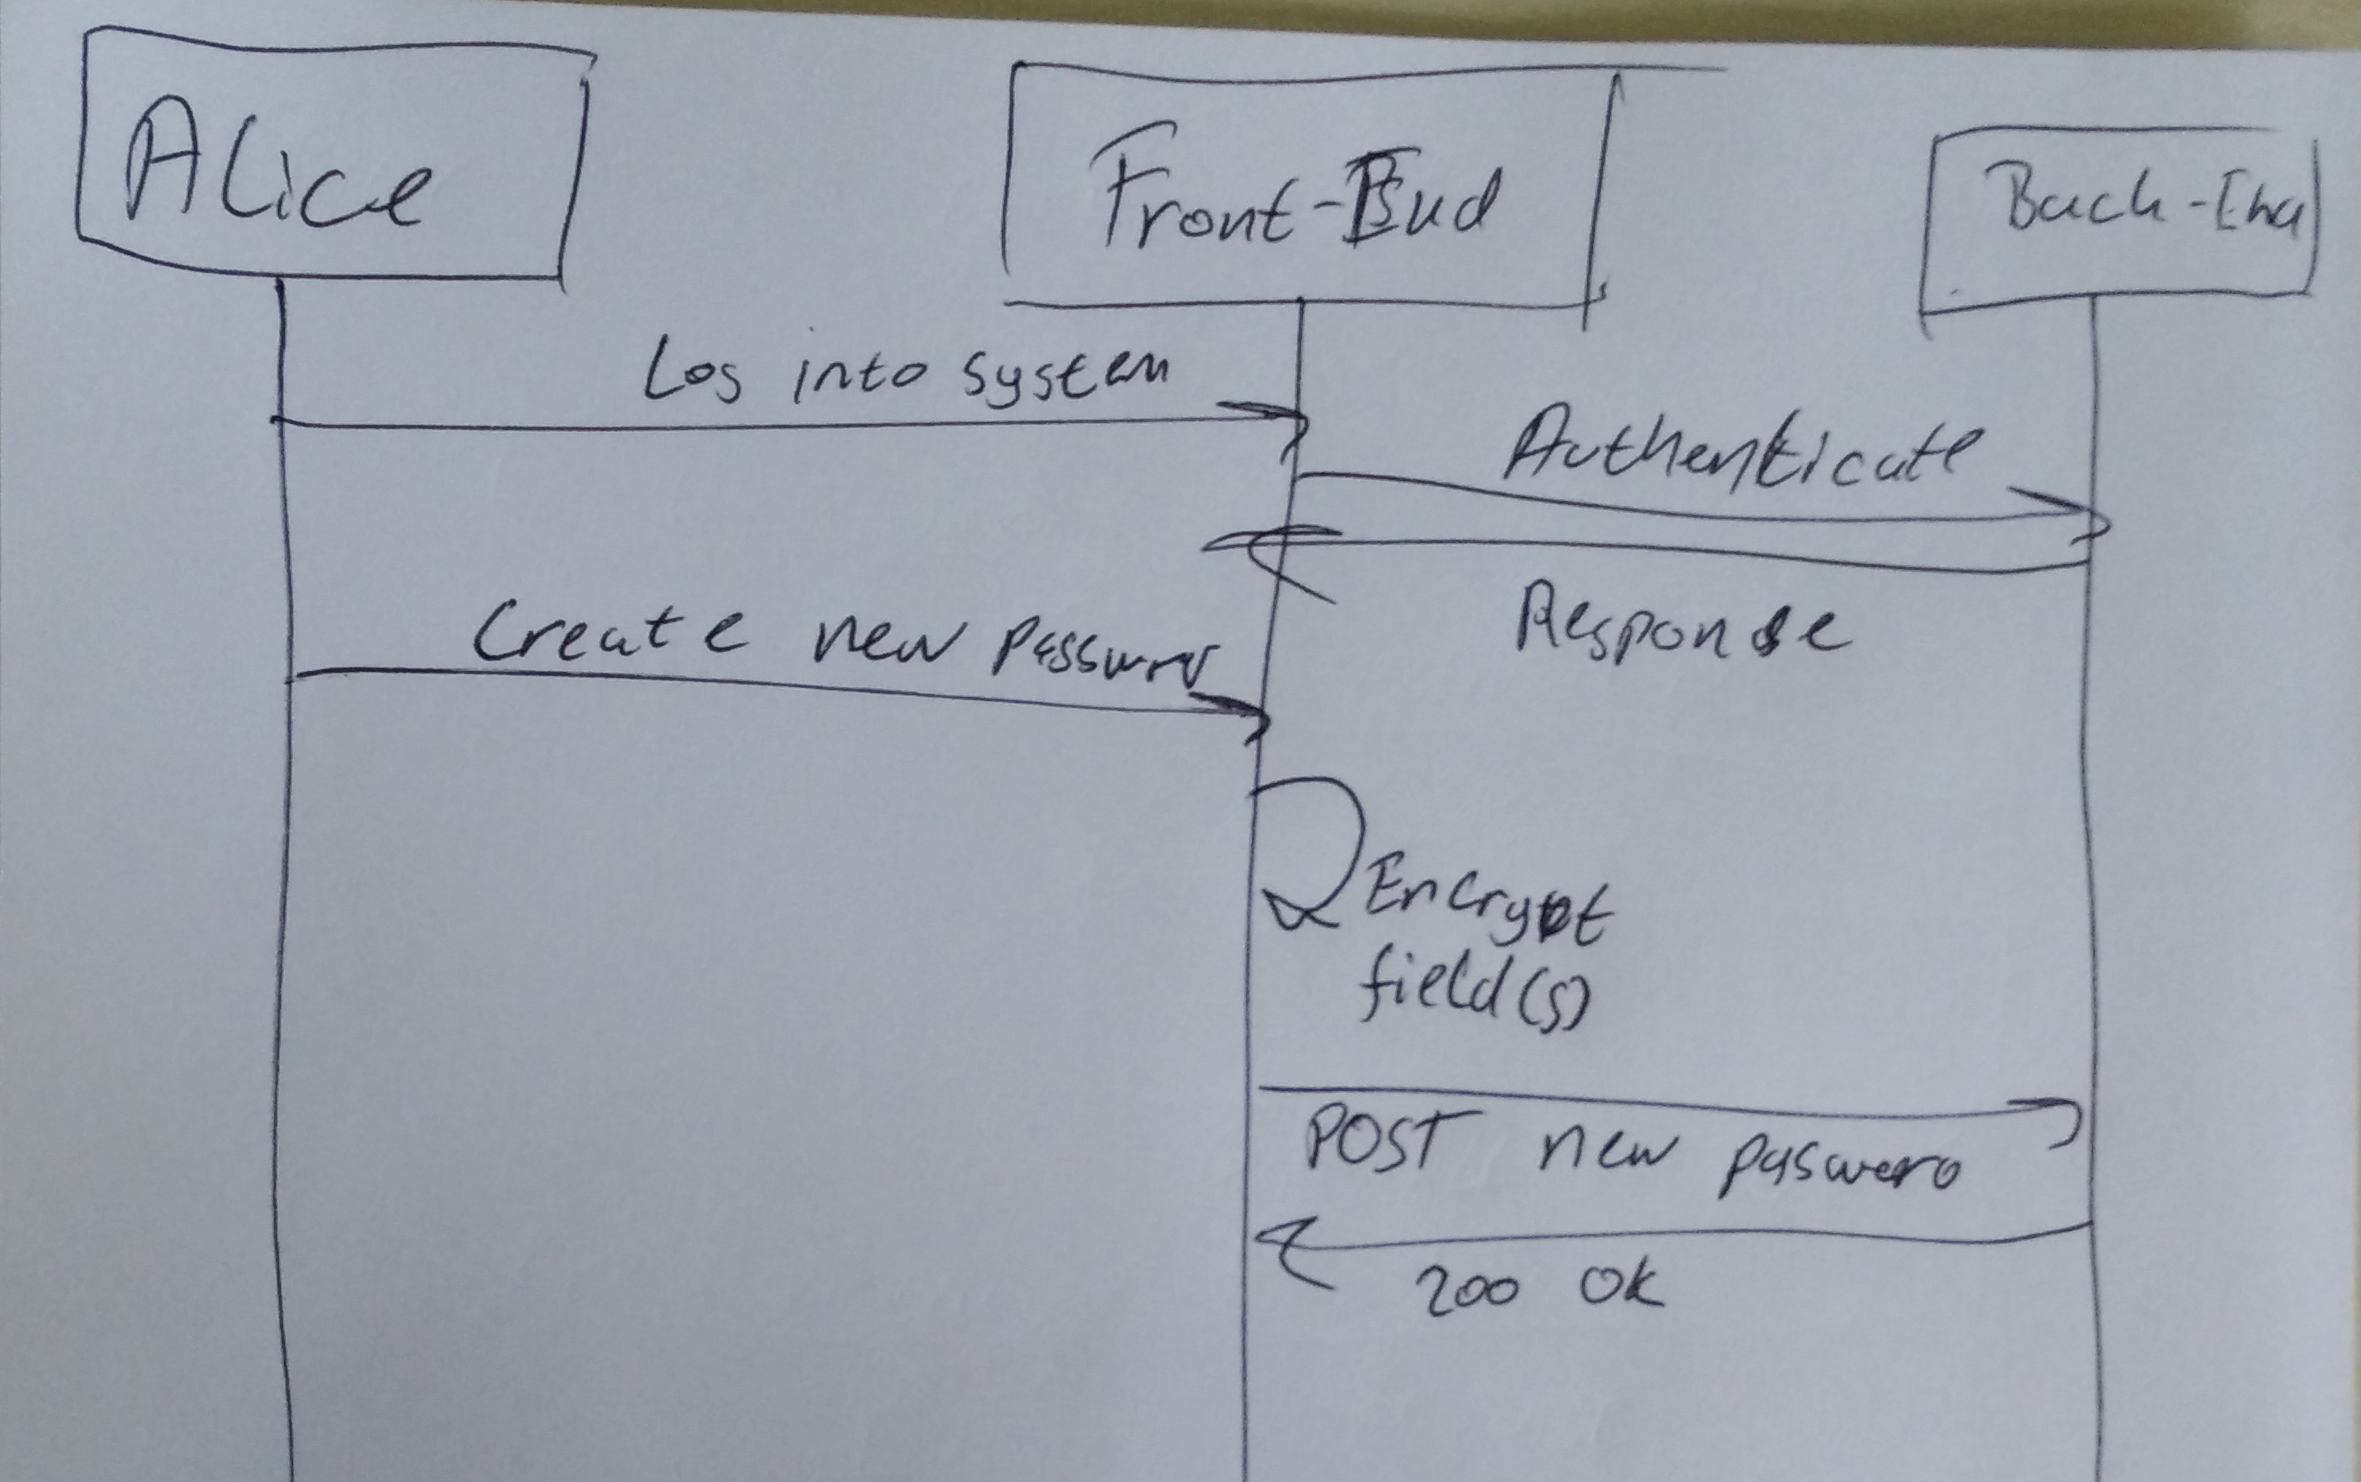
\includegraphics[width=\textwidth]{figures/design/sequence_perEntry.png}
					\caption{Squence diagram for sharing a password, when asymmetric encryption is used.}
					\label{fig:sequence:asymmetric}
				\end{figure}


				%Each user has both a private-key and a public-key stored on the server. When Alice wish to share a password with Bob, she requests the server for Bob's public-key. Once she gets this, she then re-encrypts the password with \emph{Bob's} public-key, and sends this to the server. This way, the password is never handles un-encrypted anywhere other than Alice's front-end. Finally, Bob can easily decrypt the password, using his own private-key. This sequence of events, is shown on figure \ref{fig:seq:assymetric} on page \pageref{fig:seq:assymetric}.

			\subsubsection{Making A Choice}
				\label{sec:encryption_choice}
				Having described three different approaches to solving the problem, it is time to decide exactly which should be used. All of them have their drawbacks -- all of them have their advantages. Since the asymmetric encryption approach has no acronym, it will be referred to as ``Asymmetric'' in the following tables.

				First and foremost, let us examine the availability of tools, cf. table \ref{table:comp:availability}. Admittedly, this should probably carry less weight in the design of the system, however, as mentioned earlier this \emph{will} effect the implementation heavily, should existing libraries not exist. While CL-PRE is just an example of a proxy re-encryption it is a general truth to these algorithms, that at this point in time they are more theoretical than practical -- unfortunately. In stark contrast to this, both PGP and asymmetric encryption algorithms have a plethora of implementations, for just about any combination of hardware and language available. As such, they're the clear favourites in this regard.

				\begin{table}
					\center
					\begin{tabular}{r|l}
						Solution 		& Available Implementations 	\\
						\hline
						CL-PRE 			& \red{Very Rare} 				\\
						PGP 			& \green{Several} 				\\
						Asymmetric 		& \green{Several} 				\\
					\end{tabular}
					\caption{Comparison of availability of implementations of the three encryption schemes.}
					\label{table:comp:availability}
				\end{table}

				Next, it is only fitting to compare the data requirements for these three approaches, cf. \ref{table:comp:data}. As was explained earlier, CL-PRE requires not only an encryption key stored alongside the password, but also a re-encryption key per user said password is shared to. Then there is PGP which only requires an extra encryption key \emph{per} user requiring access. Finally, there is the asymmetric approach which requires no extra data to be stored, due to it only using the users' private and public-keys. As such, the asymmetric approach is \emph{clearly} the favourite in this regard. 

				\begin{table}
					\center
					\begin{tabular}{r|l|l}
						Solution 		& Per Password Value  			& Per Share Value 	\\
						\hline
						CL-PRE 			& \red{Yes} 					& \red{Yes}			\\
						PGP 			& \green{No} 					& \red{Yes} 		\\
						Asymmetric 		& \green{No} 					& \green{No} 		\\
					\end{tabular}
					\caption{Comparison of data usage of the three encryption schemes.}
					\label{table:comp:data}
				\end{table}

				Finally, there is the matter of data processing, which is also an important aspect to take into account, cf. \ref{table:comp:data}. Creating a password with CL-PRE involves the following steps: First a symmetric DEK needs to be created, then the password is encrypted with said DEK, and finally the DEK is encrypted using the user's public-key. This totals to $3$ ``cryptographic steps''. PGP is essentially the same. First a new symmetric key is created, then the password is encrypted using that key, and finally the key is encrypted using the user's public-key. Hence, PGP also uses $3$ cryptographic steps. Using asymmetric encryption, however, only a single step is needed: Encrypt the password with the user's public-key.

				For creating a password, the asymmetric approach is clearly the favourite. Not only in the steps involved, but also just from its simplicity. However, this is not \emph{quite} the same when sharing a password. CL-PRE actually only needs a single step for updating a shared a password: Creating the re-encryption key. PGP on the other hand needs two operations: Decrypting the symmetric key, and re-encrypting it with the recipients public-key. Finally, there is the asymmetric approach. This approach needs $n$ operations, per update, where $n$ is the number of people the password is shared to. This \emph{huge} performance loss is due to the fact that it uses sharing by cloning. This is best illustrated with an example: If a password is shared with three people, it means that it exists four times in the back-end: Once encrypted with the owners public-key, and once with each of the people it is shared to. When the password is updated, it needs to be re-encrypted using \emph{each} of these peoples public-keys as well.

				In this case, it is \emph{quite} clear that the asymmetric approach is inferior, when $n$ is large. However, since this overall solution is based around individual password sharing, and not sharing between a group, it is fair to assume that $n$ will be low. As such, the performance loss significantly less than originally assumed.

				All of these three tables are combined into a single large table, on figure \ref{table:comp:complete_schemes} on page \pageref{table:comp:complete_schemes}. Looking at this table, it is quite clear that as long as the assumption of relative few shares per passwords hold, the asymmetric approach is the preferable one to use.

				\begin{table}
					\center
					\begin{tabular}{r|l|l}
						Solution 		& Creating A Password  	& Updating a Password 	\\
						\hline
						CL-PRE 			& \green{$3$} 					& \green{$1$}					\\
						PGP 			& \green{$3$} 					& \green{$2$} 					\\
						Asymmetric 		& \green{$1$}					& \red{$n$} 					\\
					\end{tabular}
					\caption{Comparison of cryptographic steps required for the three encryption schemes.}
					\label{table:comp:data}
				\end{table}



				\begin{table}
					\center
					\begin{tabular}{r|l|l|l|l|l}
						Solution 		& \rot{Available Implementations} & \rot{Storage Per Password Value}  	& \rot{Storage Per Share Value}	& \rot{Steps for Creating A Password} 	& \rot{Steps for Updating a Password} 	\\
						\hline
						CL-PRE 			& \red{Very Rare} 	& \red{Yes}		& \red{Yes} 	& \green{$3$} & \green{$1$} \\
						PGP 			& \green{Several} 	& \green{No}	& \red{Yes} 	& \green{$3$} & \green{$2$} \\
						Asymmetric 		& \green{Several} 	& \green{No}	& \green{No} 	& \green{$1$} & \yellow{$n$} \\
					\end{tabular}
					\caption{Complete comparison of the three schemes.}
					\label{table:comp:complete_schemes}
				\end{table}

		\subsection{Key Management}
			\label{sec:keys}
			As the astute reader might have realized by now, there is a slight short-coming in what has previously described. The private-key -- the key used for \emph{decrypting} passwords -- is stored on the server. If stored in ``clear text'' \emph{(or raw binary)}, this presents a huge security risk. Not only is the server admin \emph{easily} able to decrypt passwords, but \emph{should} a leak of the database happens, all passwords are instantly compromised.
			As such, it is necessary to introduce some sort of encryption for the private-key. But how can this be achieved without merely shifting the issues previously described? It is necessary to derive the encryption key, from the user's input. Translating a user's input -- for instance a password -- to an encryption key is very common, and is best done using a key derivation function. 

			Algorithms such as bcrypt and PBKDF2 exists for this very purpose \emph{(or slightly similar, at least)}. In layman's terms, it basically hashes the same password over and over again, $n$ times, as to slow the process down ``artificially''. This is done so that trying to bruteforce the key, will be several factors more difficult, due to the extra computations.

		\subsection{Comparison with Requirements}
			Having made choices regarding data encryption and protection, in the previous sections, it is now suitable to update the checklist found on figure \ref{tab:checklist_arch-comms} on page \pageref{tab:checklist_arch-comms}. Using the asymmetric approach and protecting the users' keys with a password derived symmetric key, it is clear that the following requirements are now fulfilled
			\begin{itemize}
				\item Passwords and private information should never be stored or handled un-encrypted anywhere, other than the local device
				\item Password sharing
			\end{itemize}
			As such, the checklist is updated which is reflected on figure \ref{tab:checklist_encryption} on page \pageref{tab:checklist_encryption}.

			\begin{table}
				\center
				\begin{tabular}{r l c}
													& \rot{\textbf{Fulfilled}} 	& \rot{Section(s)} \\
					\textbf{Functional} 			&						&					\\
					\hline
					\freq{item:distrib_password} 	& \green{\cmark} 		& \green{ \ref{sec:arch} \& \ref{sec:comms} }			\\
					\hline
					\freq{item:multi_user} 			& \red{\xmark} 			& \red{ }			\\
					\hline
					\freq{item:admin_user} 			& \red{\xmark} 			& \red{ }			\\
					\hline
					\freq{item:organization} 		& \red{\xmark} 			& \red{ }			\\
					\hline
					\freq{item:sharing} 			& \green{\cmark}		& \green{ \ref{sec:encryption_choice} \& \ref{sec:keys} }			\\
					\hline
					\freq{item:add} 			 	& \red{\xmark} 			& \red{ }			\\
					\hline
					\freq{item:platform} 			& \red{\xmark} 			& \red{ }			\\
					\hline
					\freq{item:database} 			& \red{\xmark} 			& \red{ }			\\
					\hline
					\freq{item:passwords_local} 	& \green{\cmark}		& \green{ \ref{sec:encryption_choice} \& \ref{sec:keys} }			\\
					\hline
					\freq{item:new} 				& \red{\xmark} 			& \red{ }			\\
					\hline
					\freq{item:retrieve} 			& \red{\xmark} 			& \red{ }			\\
					\hline
					\freq{item:delete} 				& \red{\xmark} 			& \red{ }			\\
					\hline
					\freq{item:audit} 				& \red{\xmark} 			& \red{ }			\\
					\hline
					\freq{item:auth} 				& \red{\xmark} 			& \red{ }			\\
					\hline
					\freq{item:change} 				& \red{\xmark} 			& \red{ }			\\
					\hline
					\freq{item:two-factor} 			& \red{\xmark} 			& \red{ }			\\
					\hline
					\freq{item:restart} 			& \red{\xmark} 			& \red{ }			\\
					\hline
					\textbf{Non-Functional} 		&  			 			& 					\\
					\hline
					\nfreq{item:user_storage} 		& \red{\xmark} 			& \red{ }			\\
					\hline
					\nfreq{item:open-source} 		& \red{\xmark} 			& \red{ }			\\
					\hline
					\nfreq{item:entries} 			& \red{\xmark} 			& \red{ }			\\
					\hline
					\nfreq{item:encryption} 		& \red{\xmark} 			& \red{ }			\\
					\hline
					\nfreq{item:comms} 				& \red{\xmark} 			& \red{ }			\\
					\hline
					\nfreq{item:tls1.2} 			& \red{\xmark} 			& \red{ }			\\
					\hline
					\nfreq{item:delay} 				& \red{\xmark} 			& \red{ }			\\
					\hline
				\end{tabular}

				\caption{Checklist for the requirements fulfilled so far. For a full description of the various requirements, please see section \ref{sec:requirements} on page \pageref{sec:requirements}.}
				\label{tab:checklist_encryption}
			\end{table}


	\section{Authentication}
		\subsection{OAuth1/2}
		\subsection{Basic Authentication}
		\subsection{Tokens}
			\subsubsection{Simple Web Tokens (SWT)}
			\subsubsection{JSON Web Tokens (JWT)}
		
		\subsection{Two-Factor Authentication}

	\section{Securing the API}

	\section{Encryption \& Data Security}
		\subsection{Pseudo Zero Knowledge}


	\section{Storing the Data}
		\section{SQL vs NoSQL}
	\section{Storage Scheme}

	\section{Naming the Solution}

